\paragraph{QuizziPedia::Front-End::Controllers::QuestionnaireQuestionsManagementController}
\begin{figure} [ht]
	\centering
	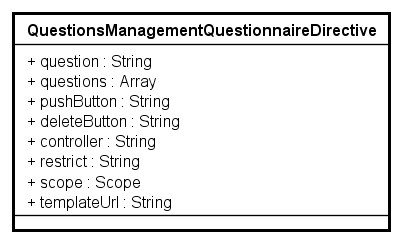
\includegraphics[scale=0.45]{UML/Classi/Front-End/QuizziPedia_Front-end_Controller_QuestionnaireQuestionsManagementController.png}
	\caption{QuizziPedia::Front-End::Controllers::QuestionnaireQuestionsManagementController}
\end{figure} \FloatBarrier
\begin{itemize}
	\item \textbf{Descrizione}: questa classe permette di gestire il recupero delle domande per il questionario;
	\item \textbf{Utilizzo}: fornisce le funzionalità per il recupero delle domande dal back-end e le rende disponibili per poter popolare le view;
	\item \textbf{Relazione con altre classi}:
	\begin{itemize}
		\item \textit{IN} \texttt{QuestionnaireQuestionsManagementDirective}: rappresenta il componente grafico che permette all'utente di:
		\begin{itemize}
			\item Effettuare delle ricerche sul database di domande;
			\item Selezionare le domande da inserire nel questionario;
			\item Mostrare le domande già inserite e permettere all'utente di eliminarle da tale lista.
		\end{itemize}
		Questo componente si presta sia per la creazione che per la modifica di un questionario;
		\item \textit{IN} \texttt{QuestionsService}: questa classe permette di ottenere domande esistenti e salvare nuove domande;
		\item \textit{IN} \texttt{QuestionItemModel}: ;
	\end{itemize}
	\item \textbf{Attributi}:
	\begin{itemize}
		\item \texttt{-} \texttt{\$scope: \$scope} \\
		Campo dati contenente un riferimento all’oggetto \$scope creato da \textit{Angular\ped{G}}, viene utilizzato come mezzo di comunicazione tra il controller e la view. Contiene gli oggetti che definiscono il model dell’applicazione;
		\item \texttt{-} \texttt{\$mdDialog: \$mdDialog} \\
		Campo dati contenente un riferimento al servizio della libreria \textit{Material for Angular\ped{G}} che permette di creare delle componenti a popup;
		\item \texttt{-} \texttt{QuestionsService: QuestionsService}\\ pParametro che permette di ottenere, tramite il service, le domande richieste;
	\end{itemize}
	\item \textbf{Metodi}:
	\begin{itemize}
		\item \texttt{+} \texttt{QuestionnaireQuestionsManagementController(\$scope: \$scope, \$mdDialog, \$mdDialog, QuestionsService: QuestionService)} \\Metodo costruttore della classe. \\
		\textbf{Parametri}:
		\begin{itemize}
			\item \texttt{-} \texttt{\$scope: \$scope} \\
			parametro contenente un riferimento all’oggetto \$scope creato da \textit{Angular\ped{G}}, viene utilizzato come mezzo di comunicazione tra il controller e la view. Contiene gli oggetti che definiscono il model dell’applicazione;
			\item \texttt{-} \texttt{\$mdDialog: \$mdDialog} \\
			Parametro contenente un riferimento al servizio della libreria \textit{Material for Angular\ped{G}} che permette di creare delle componenti a popup;
			\item \texttt{-} \texttt{QuestionsService: QuestionsService}\\ Parametro che permette di ottenere, tramite il service, le domande richieste;
		\end{itemize}
		\item \texttt{-} \texttt{getQuestions(): String[]} \\
		Metodo che permette di ottenere la lista di tutte le domande.
		\item \texttt{-} \texttt{getQuestion(questionId: String): QuestionItemModel} \\
		Metodo che ritorna l'intera domanda selezionata.
		\textbf{Parametri}:
		\begin{itemize}
			\item \texttt{questionId: String}: parametro che indica l'identificativo univoco di una domanda.
		\end{itemize}
		\item \texttt{-} \texttt{addQuestion(questionId: String) : void} \\
		Metodo che permette di inserire una domanda nel questionario.
		\textbf{Parametri}:
		\begin{itemize}
			\item \texttt{questionId: String}: parametro che indica l'identificativo univoco di una domanda.
		\end{itemize}
	\end{itemize}
\end{itemize}
